 \documentclass[t]{beamer}
%\documentclass{beamer}
\listfiles

\mode<presentation>
{
  \usetheme[deutsch,titlepage0]{KIT}
% \usetheme[usefoot]{KIT}
% \usetheme{KIT}

%%  \usefonttheme{structurebold}

  \setbeamercovered{transparent}

  %\setbeamertemplate{enumerate items}[circle]
  \setbeamertemplate{enumerate items}[ball]

}
\usepackage{babel}
%\date{10.05.2010}
%\DateText

\newlength{\Ku}
\setlength{\Ku}{1.43375pt}

\usepackage[latin1]{inputenc}
\usepackage[TS1,T1]{fontenc}
\usepackage{array}
\usepackage{multicol}
\usepackage{lipsum}

%\usenavigationsymbols
%\usenavigationsymbols[sfHhdb]
%\usenavigationsymbols[sfhHb]

\title[]{Gemeinsam an die Spitze}
%\subtitle{Karlsruhe Institute of Technology (KIT)}

\author[]{KIT}

\AuthorTitleSep{\relax}

\institute[]{KARLSRUHER INSTITUT F�R TECHNOLOGIE (KIT)}

\TitleImage[width=\titleimagewd]{Bilder/KIT-Titel}

\newlength{\tmplen}

\newcommand{\verysmall}{\fontsize{6pt}{8.6pt}\selectfont}

\begin{document}

\begin{frame}
  \maketitle
\end{frame}

\begin{frame}
  \frametitle{Eine einzigartige Kooperation}

  Karlsruher Institut f�r Technologie (KIT):
  \settowidth{\tmplen}{Forschungszentrum Karlsruhe GmbH}
  \vspace{5mm}

  \begin{columns}[onlytextwidth,b]
    \column{\tmplen}
    Die Kooperation von\\
    Forschungszentrum Karlsruhe GmbH\\
    und Universit�t Karlsruhe (TH)\\
    \mbox{}
    \addtolength{\tmplen}{-\textwidth}
    \setlength{\tmplen}{-\tmplen}
    \column{.8\tmplen}
    \hspace*{-.2\tmplen}\hfill
\includegraphics[width=\tmplen]
      {Bilder/KIT-Kooperation}
  \end{columns}
\end{frame}

\begin{frame}
  \frametitle{Zwei starke Partner}

  \small
  \renewcommand{\baselinestretch}{.95}\selectfont
  \begin{minipage}{.625\linewidth}
    \heading{Forschungszentrum Karlsruhe:}
    \begin{itemize}
    \item Programmorientierte Forschung auf h�chstem internationalem Niveau
    \item Eine der gr��ten und erfolgreichsten Forschungseinrichtungen  
          in den Natur- und Ingenieurwissenschaften in Europa
    \item Mitglied der Helmholtz-Gemeinschaft nationaler Forschungszentren
    \end{itemize}

    \heading{Universit�t Karlsruhe (TH):}
    \begin{itemize}
    \item Gewinner der Excellence Initiative 2006 der Bundesrepublik
          Deutschland und der Bundesl�nder
    \item Eine der in der Forschung bedeutendsten Universit�ten weltweit
    \item H�chste Einwerbung von Drittmitteln von der DFG pro Kopf in
          Deutschland
    \end{itemize}
  \end{minipage}
  \hfill
  \parbox{.325\linewidth}{\makebox[.325\textwidth][r]{
      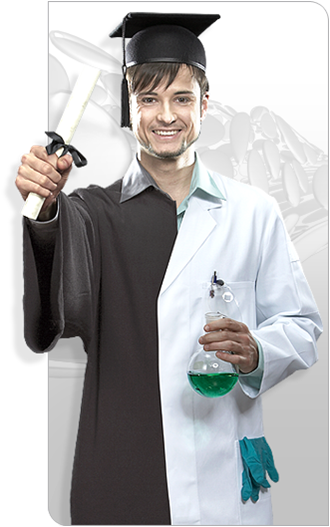
\includegraphics[width=.375\textwidth]
        {Bilder/KIT-Promotion}}}
\end{frame}

\begin{frame}
  \frametitle{Gemeinsames Ziel}

  Positionierung als Institution international herausragender Forschung
  und Lehre in den Natur-und Ingenieurwissenschaften mit wissenschaftlicher
  Exzellenz und Weltspitzenniveau in:
  \bigskip

  \setlength{\tmplen}{.2875\linewidth}
  \begin{columns}[onlytextwidth]
    \begin{column}{\tmplen}
      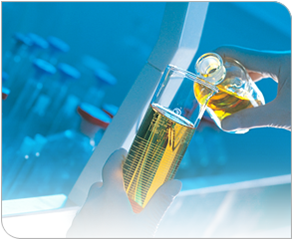
\includegraphics[width=\tmplen]
        {Bilder/KIT-Research}
      \begin{itemize}\item Forschung\end{itemize}
    \end{column}
    \begin{column}{\tmplen}
      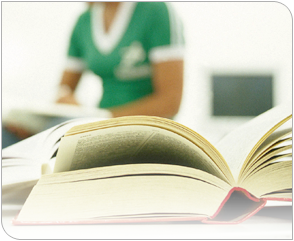
\includegraphics[width=\tmplen]
        {Bilder/KIT-Teaching}
      \begin{itemize}\item Lehre\end{itemize}
    \end{column}
    \begin{column}{\tmplen}
      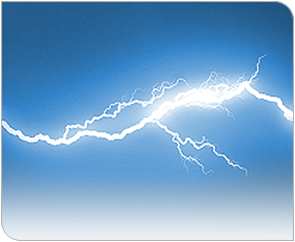
\includegraphics[width=\tmplen]
        {Bilder/KIT-Innovation}
      \begin{itemize}\item Innovation\end{itemize}
    \end{column}
  \end{columns}
  \bigskip

  \small
  Voraussetzung:\\
  ausgezeichnete Infrastruktur und hervorragende Dienstleistungseinheiten.
\end{frame}

\begin{frame}
  \frametitle{Forschungsportfolio}

  \parbox{.64\textwidth}{\raggedright
    Exzellente Forschung basiert in erster Linie auf den F�higkeiten und
    Kenntnissen der wissenschaftlichen Mitarbeiter.
    \bigskip

    In KIT ordnen sich die Wissenschaftler entsprechend ihrem Fachwissen
    Kompetenzfeldern zu, die thematisch zu Kompetenzbereichen geb�ndelt sind.
    \bigskip

    Kompetenzfelder und Kompetenzbereiche bilden das Kompetenzportfolio
    des KIT, das auch neue wissenschaftliche Fragestellungen aufgreift
    und sich so dynamisch weiterentwickelt.}
  \hfill
  \parbox{.312\textwidth}{%
    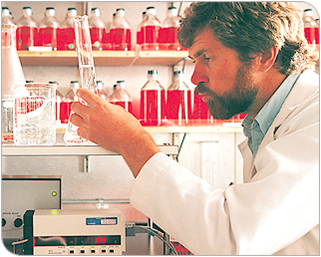
\includegraphics[width=.312\textwidth]
      {Bilder/KIT-Labor1}\\
    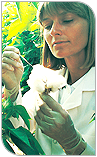
\includegraphics[width=.133\textwidth]
      {Bilder/KIT-Labor2}
    \hfill
    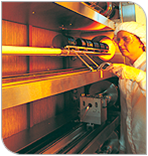
\includegraphics[width=.176\textwidth]
      {Bilder/KIT-Labor3}}
\end{frame}

\begin{frame}
  \frametitle{Kompetenzportfolio}
  \framesubtitle{\normalsize\mdseries 30 Kompetenzfelder geb�ndelt in 6 Kompetenzbereiche}

  \renewcommand{\baselinestretch}{.8}\verysmall
  \begin{tikzpicture}
    % Materie und Materialien
    \draw[KITblack50,fill=KITblack30,line width=.5\Ku]
      (0\Ku,135\Ku) rectangle
      (76\Ku,126\Ku)
      (38\Ku,130.5\Ku) node {\color{black}Materie und Materialien};
    \draw[KITblack50,fill=KITblack15,line width=.5\Ku]
      (0\Ku,126\Ku) rectangle
      (76\Ku,87\Ku);
    \pgftext[at=\pgfpoint{0\Ku}{124.6\Ku},top,left]{%
      \parbox{74\Ku}{%
        \begin{itemize}\verysmall\itemsep=0pt\parsep=0pt
        \item Elementarteilchen- und Astroteilchenphysik
        \item Kondensierte Materie
        \item Nanowissenschaft
        \item Mikrotechnologie
        \item Optik und Photonik
        \item Angewandte und neue Materialien
        \end{itemize}}}
    % Erde und Umwelt
    \draw[KITblack50,fill=KITblack30,line width=.5\Ku]
      (79\Ku,135\Ku) rectangle
      (155\Ku,126\Ku)
      (119\Ku,130.5\Ku) node {\color{black}Erde und Umwelt};
    \draw[KITblack50,fill=KITblack15,line width=.5\Ku]
      (79\Ku,126\Ku) rectangle
      (155\Ku,87\Ku);
    \pgftext[at=\pgfpoint{79\Ku}{128.5\Ku},top,left]{%
      \parbox{74\Ku}{%
        \begin{itemize}\verysmall\itemsep=0pt\parsep=0pt
        \item Atmosph�ren und Klima
        \item Geosph�re und Risikomanagement
        \item Hydrosph�re und Umwelttechnologie
        \item Bauwerke und urbane Infrastruktur
        \end{itemize}}}
    % Angewandte Lebenswissenschaften
    \draw[KITblack50,fill=KITblack30,line width=.5\Ku]
      (158\Ku,135\Ku) rectangle
      (230\Ku,126\Ku)
      (194\Ku,130.5\Ku) node {\color{black}Angewandte Lebenswissenschaften};
    \draw[KITblack50,fill=KITblack15,line width=.5\Ku]
      (158\Ku,126\Ku) rectangle
      (230\Ku,87\Ku);
    \pgftext[at=\pgfpoint{158\Ku}{128.5\Ku},top,left]{%
      \parbox{74\Ku}{%
        \begin{itemize}\verysmall\itemsep=0pt\parsep=0pt
        \item Biotechnologie
        \item Toxikologie und Ern�hrungswissenschaft
        \item Gesundheit und Medizintechnik
        \item Zell- und Strukturbiologie
        \end{itemize}}}
    % Systeme undProzesse
    \draw[KITblack50,fill=KITblack30,line width=.5\Ku]
      (0\Ku,84\Ku) rectangle
      (230\Ku,75\Ku)
      (115\Ku,79.5\Ku) node {\color{black}Systeme undProzesse};
    % links:
    \draw[KITblack50,fill=KITblack15,line width=.5\Ku]
      (0\Ku,75\Ku) rectangle
      (115\Ku,51\Ku);
    \pgftext[at=\pgfpoint{4\Ku}{77.0\Ku},top,left]{%
      \parbox{107\Ku}{%
        \begin{itemize}\verysmall\itemsep=0pt\parsep=0pt
        \item Str�mungs-und Partikeldynamik
        \item Chemische und Thermische Verfahrenstechnik
        \item Brennstoffe und Verbrennung
        \end{itemize}}}
    % rechts:
    \draw[KITblack50,fill=KITblack15,line width=.5\Ku]
      (115\Ku,75\Ku) rectangle
      (230\Ku,51\Ku);
    \pgftext[at=\pgfpoint{119\Ku}{77.0\Ku},top,left]{%
      \parbox{107\Ku}{%
        \begin{itemize}\verysmall\itemsep=0pt\parsep=0pt
        \item Systeme und eingebettete Systeme
        \item Kraftwerkstechnik
        \item Produktlebenszyklus
        \item Mobile Systeme und Mobilit�t
        \end{itemize}}}
    % Information, Kommunikation und Organisation
    \draw[KITblack50,fill=KITblack30,line width=.5\Ku]
      (0\Ku,48\Ku) rectangle
      (111\Ku,39\Ku)
      (55.5\Ku,43.5\Ku) node {\color{black}Information, Kommunikation
        und Organisation};
    \draw[KITblack50,fill=KITblack15,line width=.5\Ku]
      (0\Ku,39\Ku) rectangle
      (111\Ku,4\Ku);
    \pgftext[at=\pgfpoint{2\Ku}{41.0\Ku},top,left]{%
      \parbox{109\Ku}{%
        \begin{itemize}\verysmall\itemsep=0pt\parsep=0pt
        \item Algorithmen, Software und Informatiksysteme
        \item Kognitive Systeme und Informationsverarbeitung
        \item Kommunikationstechnik 
        \item Hochleistungsrechnen und Verteilte Systeme
        \item Mathematische Modelle
        \item Organisations-und Dienstleistungsgestaltung
        \end{itemize}}}
    % Technik, Kultur und Gesellschaft
    \draw[KITblack50,fill=KITblack30,line width=.5\Ku]
      (119\Ku,48\Ku) rectangle
      (230\Ku,39\Ku)
      (174.5\Ku,43.5\Ku) node {\color{black}Technik, Kultur und Gesellschaft};
    \draw[KITblack50,fill=KITblack15,line width=.5\Ku]
      (119\Ku,39\Ku) rectangle
      (230\Ku,4\Ku);
    \pgftext[at=\pgfpoint{121\Ku}{41.0\Ku},top,left]{%
      \parbox{109\Ku}{%
	\begin{itemize}\verysmall\itemsep=0pt\parsep=0pt
	\item Kulturerbe und sozialer Wandel
	\item Wirtschaftsorganisation und Innovation
	\item Wechselwirkung von Wissenschaft, Technik und Gesellschaft
	\end{itemize}}}
  \end{tikzpicture}
  \renewcommand{\baselinestretch}{1}\selectfont
\end{frame}

\begin{frame}
  \frametitle{Zentren und Schwerpunkte}
  \framesubtitle{\mdseries Thematische Orientierung, strategische
    Forschungsplanung}

  \parbox{.65\textwidth}{%
    KIT-Zentren:
    \begin{itemize}
      \item Energie
      \item NanoMikro
      \item Elementarteilchen-und Astroteilchenphysik
      \item Klima und Umwelt
    \end{itemize}
    \bigskip

    KIT-Schwerpunkte:
    \begin{itemize}
      \item COMMputation
      \item Mobilit�tssysteme
      \item Optik und Photonik
      \item Mensch und Technik
      \item Neue und angewandte Materialien
    \end{itemize}}
  \hfill
  \parbox{.3\textwidth}{%
    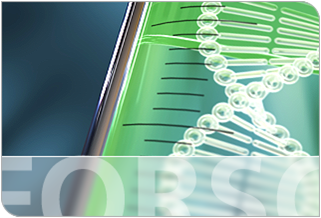
\includegraphics[width=.3\textwidth]
      {Bilder/KIT-Zentren}\\
    \parbox{.135\textwidth}{%
    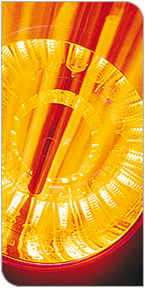
\includegraphics[width=.14\textwidth]
      {Bilder/KIT-Schwerpunkt1}}%
    \hfill
    \parbox{.149\textwidth}{%
      \hspace*{-.005\textwidth}%
      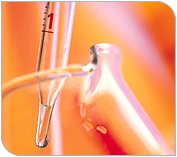
\includegraphics[width=.154\textwidth]
        {Bilder/KIT-Schwerpunkt2}\\
      \hspace*{-.005\textwidth}%
      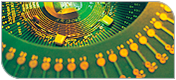
\includegraphics[width=.154\textwidth]
        {Bilder/KIT-Schwerpunkt3}
      \vspace*{.055\textwidth}}}
\end{frame}

\begin{frame}
  \frametitle{KIT in Zahlen}

  \vspace*{10\Ku}
  \begin{tabular}[b]{r}
    Mitarbeiter \\
    \resizebox{68\Ku}{!}{\bfseries\color{KITgreen}8.000}
  \end{tabular}
  \hfill
  \begin{tabular}[b]{r@{\hspace{-.2em}}l}
    & Studierende \\
    \resizebox{100\Ku}{!}{\bfseries\color{KITblack50}19.895}
  \end{tabular}\\[-1\Ku]
  \hfill
  \raisebox{7\Ku}{%
    \begin{tabular}{r}
      \resizebox{52\Ku}{!}{\bfseries 350\phantom{0}} \\
      Professoren
    \end{tabular}}
  \hspace{1\Ku}
  \begin{tabular}{l}
    \resizebox{72\Ku}{!}{\bfseries\color{KITgreen}650} \\
    \hspace*{12.5\Ku}Millionen Euro Jahresbudget
  \end{tabular}
  \bigskip

  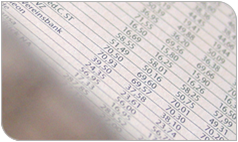
\includegraphics[height=35\Ku]{Bilder/KIT-Liste1}
  \hspace{1\Ku}
  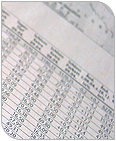
\includegraphics[height=35\Ku]{Bilder/KIT-Liste2}
\end{frame}

\begin{frame}
  \frametitle{Karlsruher Institut f�r Technologie}

  \vspace*{10\Ku}
  Danke f�r Ihre Aufmerksamkeit.
  \bigskip

  
\includegraphics[width=\textwidth]{Bilder/KIT-Finale-c}
\end{frame}
\end{document}
